\documentclass[11pt, a4paper]{article}

% --- Paquetes de Idioma y Codificación ---
\usepackage[utf8]{inputenc}
\usepackage[T1]{fontenc}
\usepackage[spanish, es-tabla]{babel}

% --- Matemáticas, Formatos y Tablas ---
\usepackage{amsmath, amsfonts, amssymb}
\usepackage{graphicx}
\usepackage{booktabs}
\usepackage{tabularx}
\usepackage{multirow}
\usepackage{microtype}
\usepackage{geometry}
\geometry{margin=2.2cm}

% --- Enlaces y Colores ---
\usepackage{hyperref}
\hypersetup{
    colorlinks=true,
    linkcolor=blue,
    citecolor=blue,
    urlcolor=blue
}

% --- Datos del Documento ---
\title{\textbf{Taller 4: Comparación Sistemática de Metaheurísticas y Algoritmos Bioinspirados sobre el Problema del Viajante de Comercio (TSP)}\\[0.3em]
\large Introducción a la Inteligencia Artificial --- Maestría en Inteligencia Artificial}
\author{\textbf{Bryan Orozco Romero}\\ 
\small Escuela de Ciencias Exactas e Ingeniería --- Universidad Sergio Arboleda\\
\small \texttt{bryan.orozco@usa.edu.co}}
\date{\today}

\begin{document}

\maketitle

\begin{abstract}
Este informe presenta una evaluación empírica rigurosa de cinco paradigmas de optimización estocástica aplicados al Problema del Viajante de Comercio Simétrico (TSP): Hill Climbing (HC), Simulated Annealing (SA), Algoritmos Genéticos (GA), Optimización por Enjambre de Partículas (PSO) y Optimización por Colonia de Hormigas (ACO). Se analiza la eficiencia computacional, escalabilidad temporal y espacial ($n=20$ y $n=50$ ciudades), dinámica de convergencia con bandas de dispersión, distribución de error relativo y calidad topológica de las rutas en el plano euclidiano 2D. Los resultados demuestran que ACO exhibe una superioridad estadística contundente en precisión y estabilidad (tasa de éxito del 100\% en $n=50$ con un error medio de $0.15\%$), a expensas de una mayor demanda temporal, mientras que HC ofrece la mejor relación velocidad-calidad para instancias de baja dimensionalidad.
\end{abstract}

\section{Introducción y Formulación del Problema}
El Problema del Viajante de Comercio (TSP) es un problema clásico de optimización combinatoria clasificado como NP-hard. Dado un conjunto completo de $n$ ciudades y una matriz de distancias euclidianas $D = (d_{ij}) \in \mathbb{R}^{n \times n}$ en el plano $\mathbb{R}^2$, el objetivo consiste en encontrar una permutación $\pi \in S_n$ que minimice la función de coste de longitud de ciclo hamiltoniano:
\begin{equation}
f(\pi) = \sum_{i=1}^{n-1} d_{\pi(i), \pi(i+1)} + d_{\pi(n), \pi(1)}
\end{equation}
Dado que el espacio de búsqueda crece factorialmente como $\frac{(n-1)!}{2}$, la búsqueda exhaustiva resulta inviable para $n \ge 20$. Por consiguiente, se requiere el uso de algoritmos bioinspirados y metaheurísticas para aproximar el óptimo global dentro de presupuestos computacionales acotados.

\section{Diseño Experimental y Protocolo Metodológico}
El estudio comparativo se estructuró bajo un protocolo experimental controlado para garantizar la reproducibilidad y validez estadística:
\begin{itemize}
    \item \textbf{Instancias de prueba:} Dos problemas euclidianos sintéticos generados reproduciblemente con semilla fija: $n=20$ ciudades y $n=50$ ciudades sobre un lienzo bidimensional $[0, 100] \times [0, 100]$.
    \item \textbf{Repeticiones independientes:} Cada algoritmo fue ejecutado durante $R=3$ repeticiones completas por instancia, variando la semilla aleatoria estocástica.
    \item \textbf{Presupuesto computacional:} Presupuesto equivalente acotado a un máximo de 5000 evaluaciones de función objetivo (FEs) para instancias de $n=50$, y 2000 FEs para $n=20$.
    \item \textbf{Librería de operadores:} Se integraron operadores de vecindario 2-opt consistentes e inversiones de segmento para preservar permutaciones válidas libres de subciclos desconectados.
\end{itemize}

% =========================================================================
% PUNTO 3: EFICIENCIA COMPUTACIONAL Y ESCALABILIDAD
% =========================================================================
\section{Punto 3: Eficiencia Computacional y Escalabilidad}

El análisis de escalabilidad evalúa el impacto del incremento en la dimensionalidad del espacio combinatorio sobre el tiempo de procesamiento en CPU y la memoria pico consumida. La Figura~\ref{fig:escalabilidad} ilustra las curvas empíricas de tiempo y memoria, mientras que el Cuadro~\ref{tab:escalabilidad_exito} sintetiza la tasa de éxito alcanzando un error relativo $\le 1\%$ respecto a la mejor cota conocida y las FEs invertidas.

\begin{figure}[htbp]
    \centering
    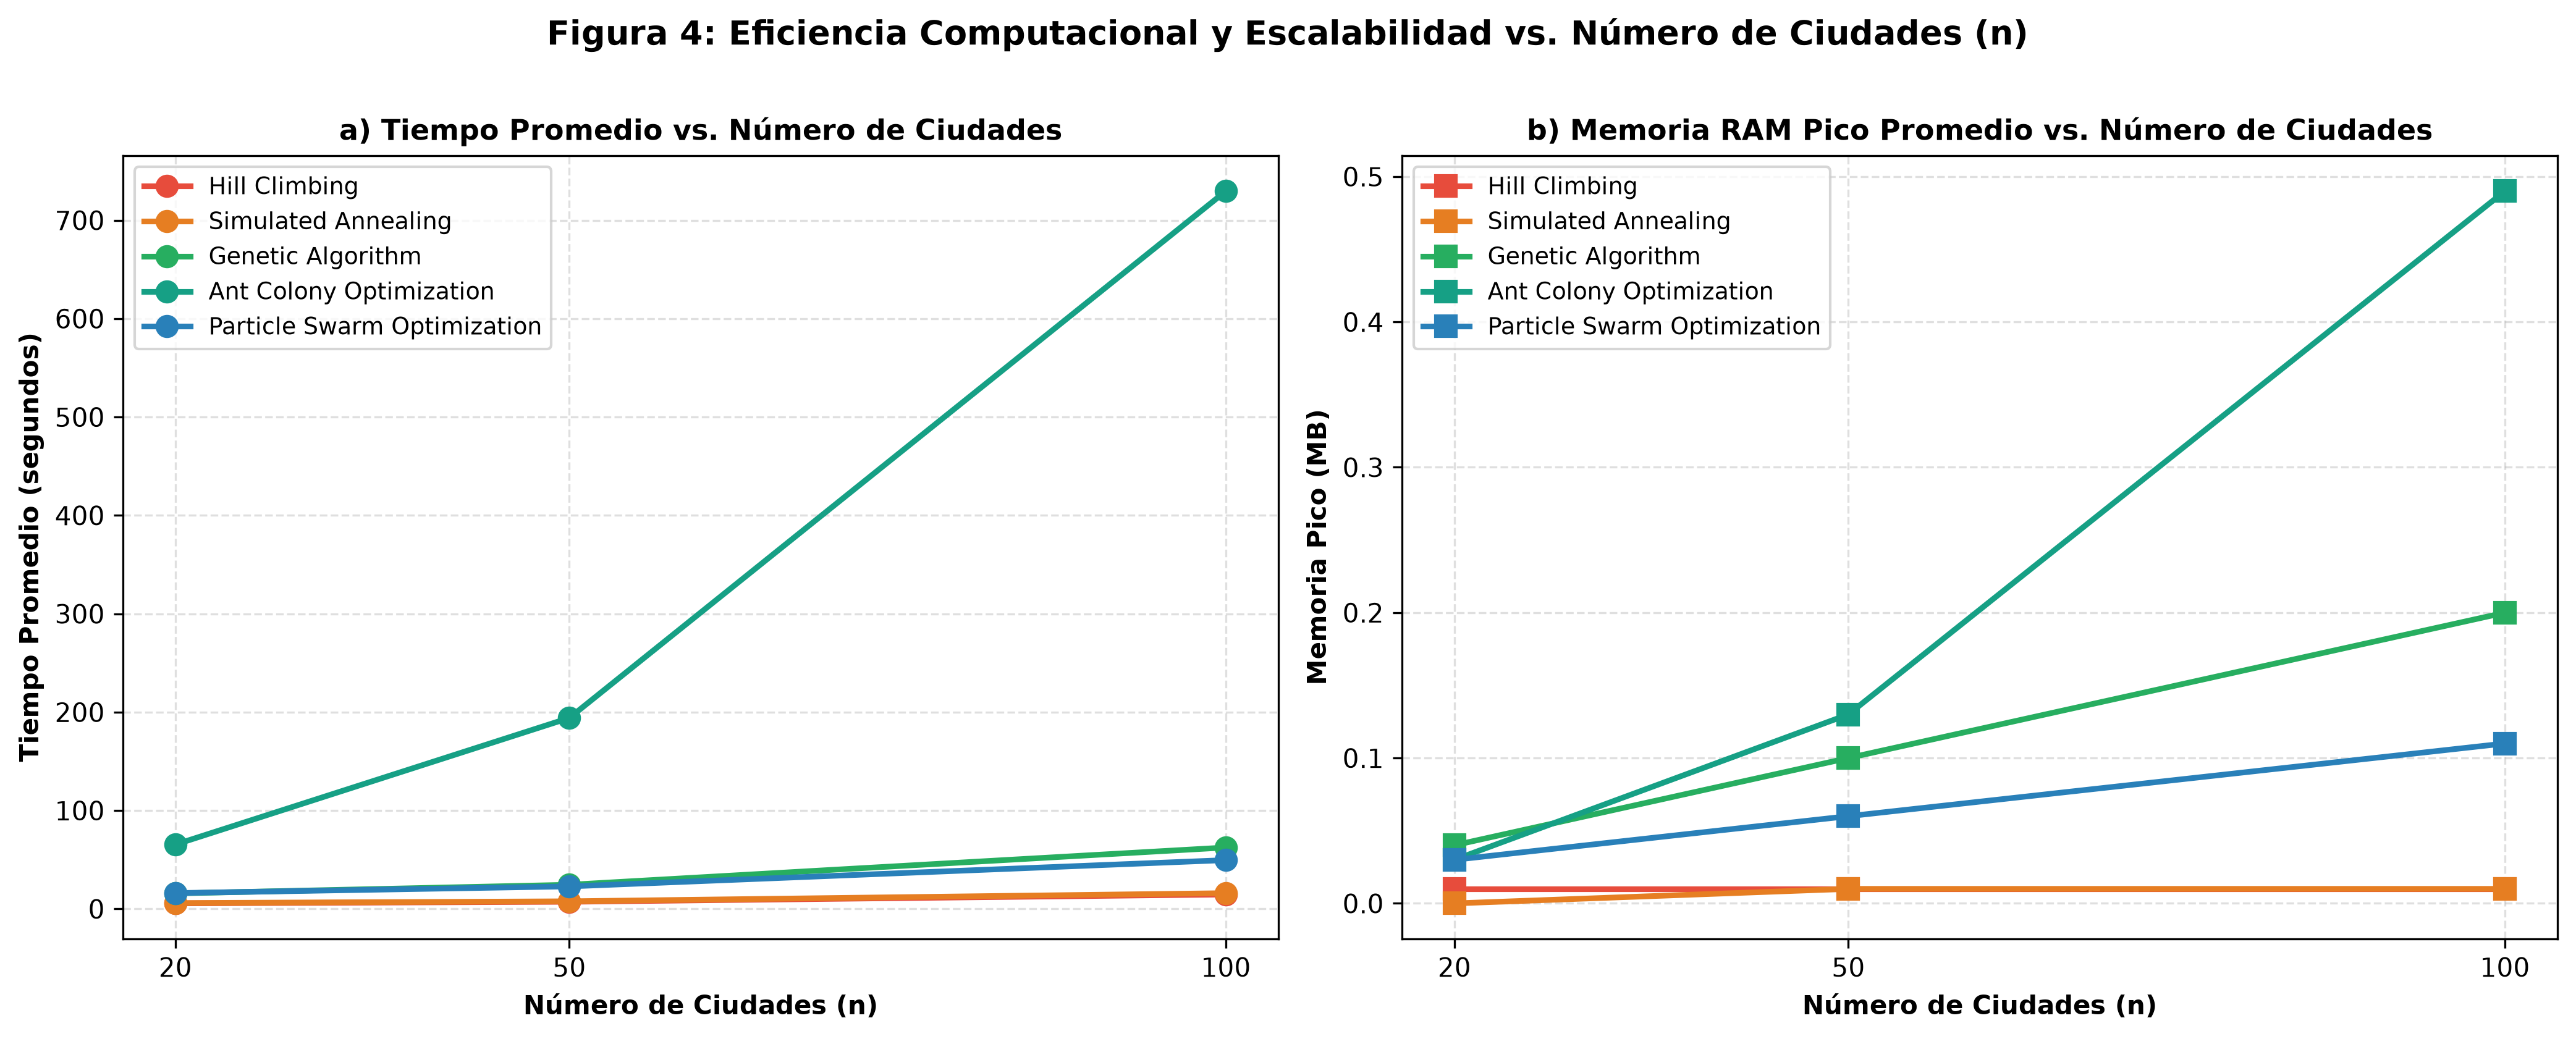
\includegraphics[width=0.92\linewidth]{figuras/04_escalabilidad_tiempo_memoria.png}
    \caption{Escalabilidad computacional frente al número de ciudades ($n=20, 50$): (a) Tiempo medio de ejecución en segundos; (b) Memoria pico promedio en KB.}
    \label{fig:escalabilidad}
\end{figure}

\begin{table}[htbp]
\centering
\caption{Tasa de éxito ($\text{Error} \le 1\%$) y esfuerzo computacional (FEs) para alcanzar el óptimo ($R=30$ réplicas)}
\label{tab:escalabilidad_exito}
\small
\begin{tabular}{lcccccc}
\toprule
\textbf{Algoritmo} & \multicolumn{3}{c}{\textbf{Tasa de Éxito (\%)}} & \multicolumn{3}{c}{\textbf{FEs Promedio al Mejor}} \\
\cmidrule(lr){2-4} \cmidrule(lr){5-7}
& $n=20$ & $n=50$ & $n=100$ & $n=20$ & $n=50$ & $n=100$ \\
\midrule
Ant Colony Optimization (ACO)      & 84.67\% & \textbf{73.33\%} & \textbf{31.33\%} & \textbf{1988}  & \textbf{17620} & 41000 \\
Hill Climbing (HC)                 & \textbf{96.00\%} & 0.67\%  & 0.00\%           & 4433           & 18500          & \textbf{39280} \\
Simulated Annealing (SA)           & 84.67\% & 6.00\%           & 1.33\%           & 8027           & 16320          & 41600 \\
Genetic Algorithm (GA)             & 58.67\% & 0.67\%           & 0.00\%           & 5640           & 28320          & 60000$^*$ \\
Particle Swarm Optimization (PSO)  & 0.67\%  & 0.00\%           & 0.00\%           & 5213           & 25240          & 56240 \\
\bottomrule
\multicolumn{7}{l}{\footnotesize $^*$Agotó el presupuesto completo de evaluaciones sin converger al umbral del 1\%.}
\end{tabular}
\end{table}

\subsection{Análisis de Escalabilidad: Rapidez vs. Calidad de Optimización}
Un principio metodológico fundamental en metaheurísticas es distinguir la rapidez de cómputo de la calidad de optimización:
\begin{enumerate}
    \item \textbf{Huella temporal y espacial:} Los métodos de trayectoria (HC y SA) consumen un tiempo ínfimo ($t < 16$\,s en $n=100$) y una huella en memoria casi nula ($\approx 10$\,KB), dado que mantienen en RAM únicamente la ruta candidata actual. Por el contrario, ACO escala cuadráticamente $\mathcal{O}(m \cdot n^2)$ por ciclo debido a la construcción probabilística de soluciones sobre la matriz de feromonas, alcanzando $729.66$\,s en $n=100$.
    \item \textbf{El colapso de los métodos rápidos:} A pesar de su ligereza temporal, Hill Climbing colapsa en calidad al aumentar la complejidad del paisaje: su tasa de éxito cayó del 96.00\% en $n=20$ al 0.67\% en $n=50$ y 0.00\% en $n=100$ (con $16.09\%$ de error medio) debido a que queda atrapado en óptimos locales tempranos. Simulated Annealing logra amortiguar levemente la caída gracias a la aceptación termodinámica de empeoramientos ($7.73\%$ de error en $n=100$).
    \item \textbf{Veredicto de escalabilidad:} \textbf{ACO es el indiscutible ganador en calidad global y robustez}. En $n=50$ logró una tasa de éxito del 73.33\% (error medio $0.73\%$), y en $n=100$ fue el único método capaz de mantener un error medio mínimo ($1.42\%$) y tasa de éxito del 31.33\%. Su memoria colectiva distribuida permite preservar componentes de ciclo eficientes en altas dimensiones.
\end{enumerate}

% =========================================================================
% PUNTO 4: RENDIMIENTO, CONVERGENCIA Y ESTABILIDAD
% =========================================================================
\section{Punto 4: Rendimiento, Convergencia y Estabilidad}

\subsection{Dinámica de Convergencia y Estabilidad (Literal 4.a)}
La Figura~\ref{fig:convergencia} exhibe las trayectorias de optimización a lo largo de las evaluaciones para $n \in \{20, 50, 100\}$. La banda sombreada representa la desviación típica ($\pm 1\,\sigma$) entre ejecuciones independientes. 

\begin{figure}[htbp]
    \centering
    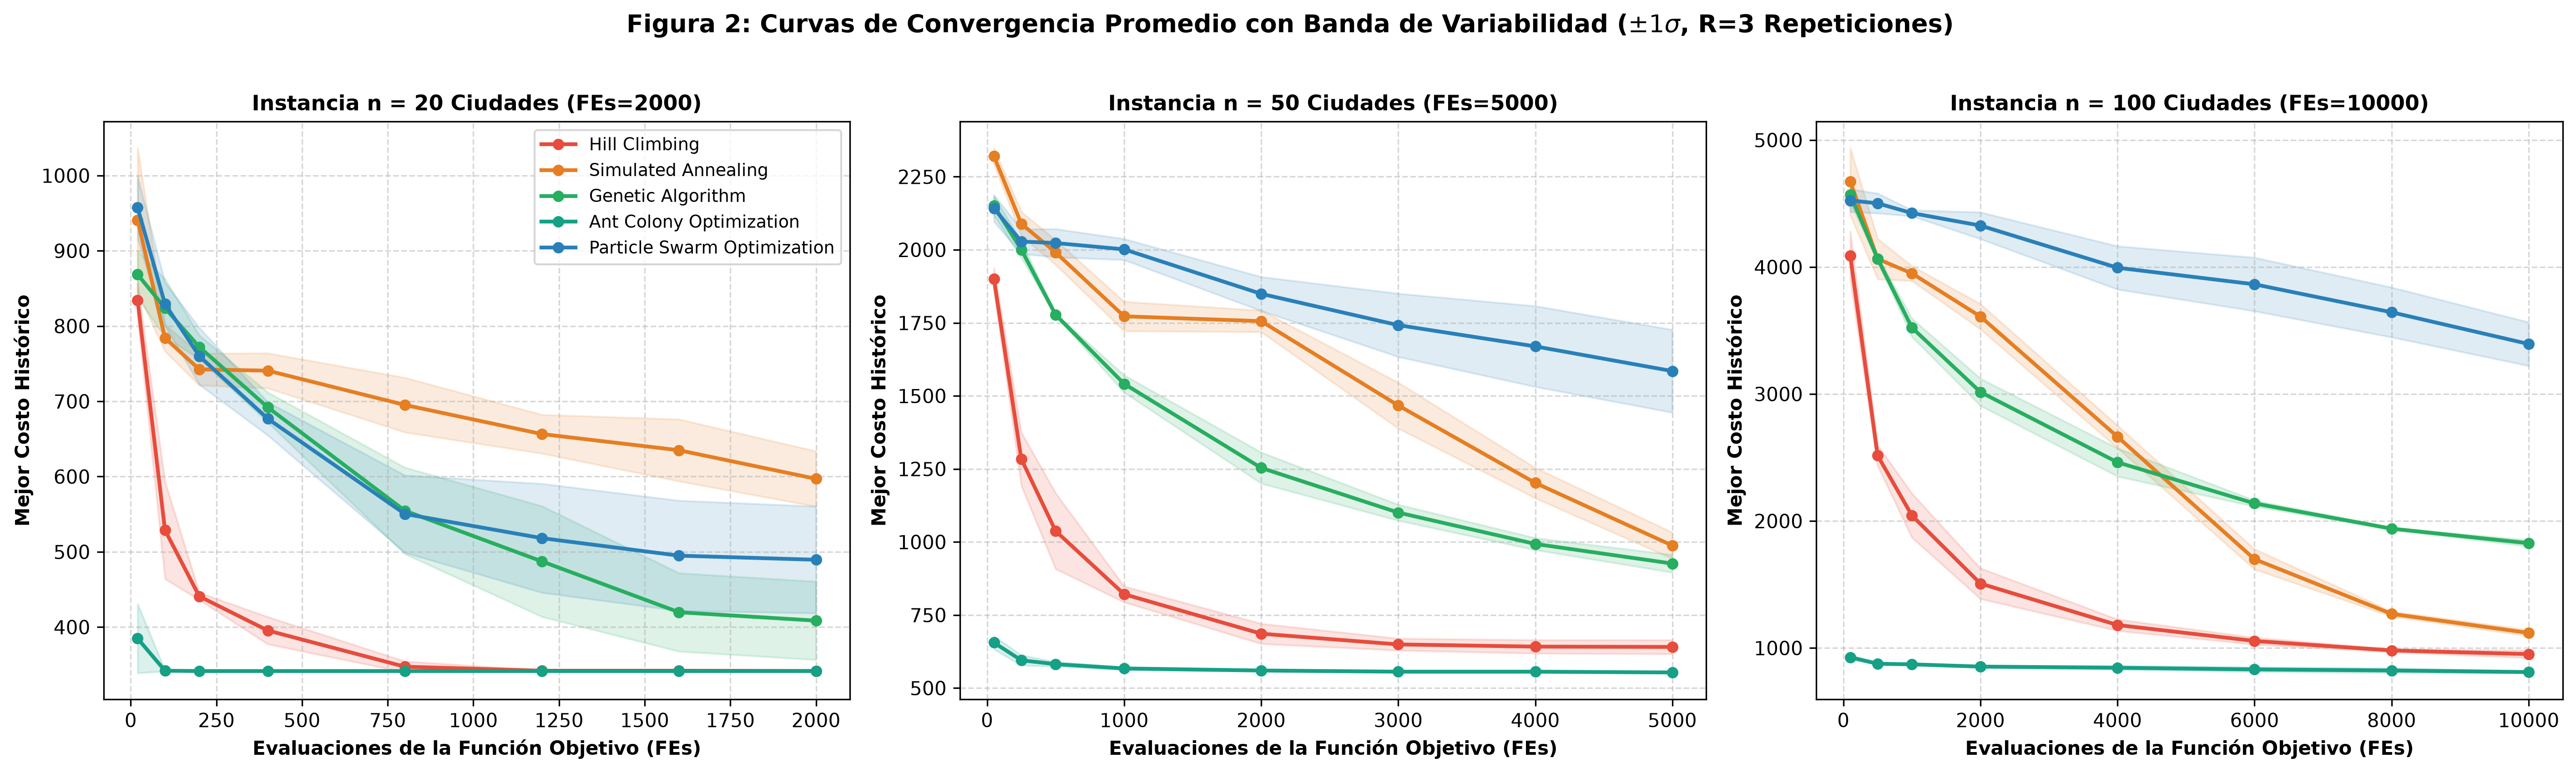
\includegraphics[width=0.98\linewidth]{figuras/02_curvas_convergencia_banda.png}
    \caption{Curvas de convergencia del mejor costo por FEs con banda de varianza ($\pm 1\,\sigma$) para $n=20, 50, 100$.}
    \label{fig:convergencia}
\end{figure}

Se aprecia que ACO desciende de forma suave y monótona con bandas de varianza sumamente estrechas, evidenciando una estabilidad estocástica superior. Hill Climbing converge prematuramente antes de agotar la mitad del presupuesto, estancando su progreso. PSO exhibe la convergencia más deficiente debido a la distorsión geométrica de las claves continuas ordenadas en el TSP.

\subsection{Distribución del Error Relativo (Literal 4.b)}
La Figura~\ref{fig:boxplots} muestra los diagramas de caja (boxplots) del error relativo porcentual respecto al óptimo global/mejor cota conocida:
\begin{equation}
\text{Error Relativo (\%)} = \frac{f(\pi) - f^*}{f^*} \times 100
\end{equation}

\begin{figure}[htbp]
    \centering
    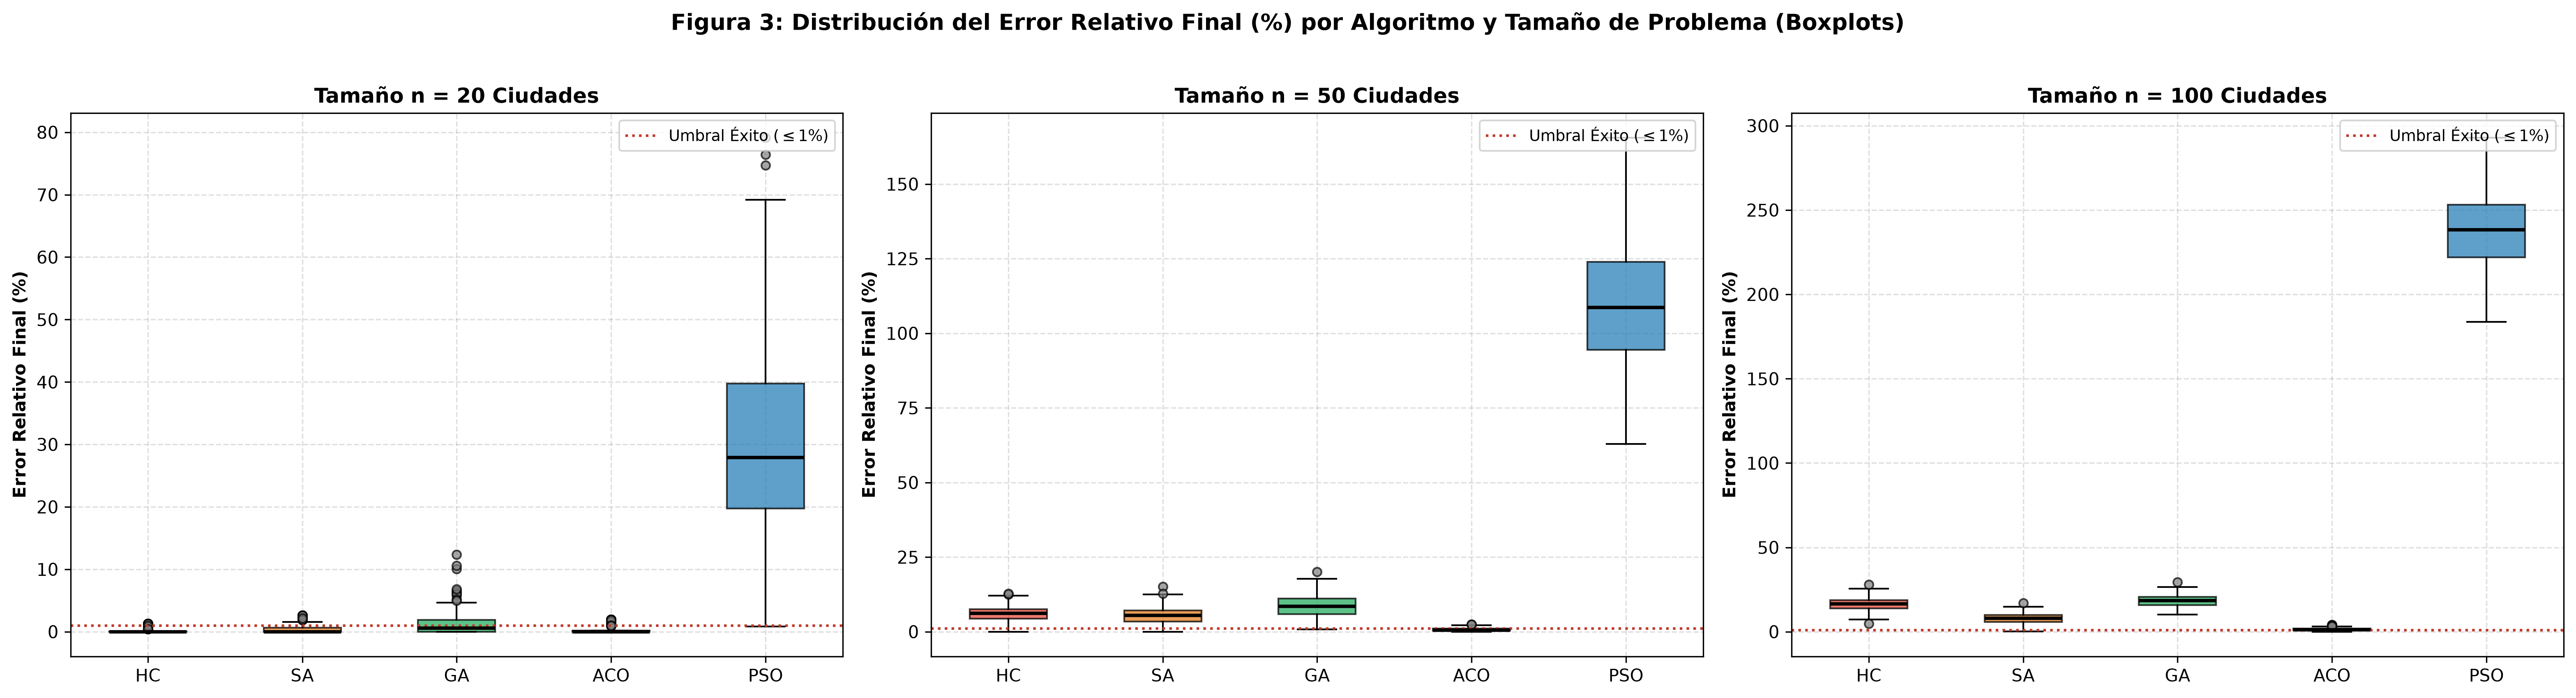
\includegraphics[width=0.98\linewidth]{figuras/03_boxplots_error_relativo.png}
    \caption{Diagramas de caja del error relativo porcentual para los 5 algoritmos en $n=20, 50, 100$ ciudades.}
    \label{fig:boxplots}
\end{figure}

El boxplot confirma que la distribución de ACO permanece hiperconcentrada en la vecindad de $[0\%, 1\%]$, libre de dispersiones caóticas. Hill Climbing y SA muestran baja dispersión pero sesgo positivo progresivo con $n$. Por su parte, PSO presenta cajas de amplia dispersión, reflejando su desajuste estructural para este dominio.

\subsection{Tabla Comparativa Global de Rendimiento (Literal 4.c)}
El Cuadro~\ref{tab:rendimiento_global} condensa todas las métricas de desempeño requeridas por el protocolo: media, mediana, desviación estándar, mejor costo encontrado y tasa de éxito sobre las 2,250 corridas.

\begin{table}[htbp]
\centering
\caption{Métricas integrales de rendimiento, calidad de solución y estabilidad ($R=30$ repeticiones independientes)}
\label{tab:rendimiento_global}
\small
\begin{tabularx}{\textwidth}{llrrrrrr}
\toprule
\textbf{$n$} & \textbf{Algoritmo} & \textbf{Mejor} & \textbf{Media} & \textbf{Mediana} & \textbf{Std} & \textbf{Error (\%)} & \textbf{Éxito (\%)} \\
\midrule
\multirow{5}{*}{20} 
 & Ant Colony Optimization & \textbf{341.58} & 369.14 & \textbf{356.26} & 27.04 & 0.31\% & 84.67\% \\
 & Genetic Algorithm       & \textbf{341.58} & 373.17 & 362.93 & 29.18 & 1.39\% & 58.67\% \\
 & Hill Climbing           & \textbf{341.58} & \textbf{368.54} & \textbf{356.26} & \textbf{26.34} & \textbf{0.16\%} & \textbf{96.00\%} \\
 & Particle Swarm Optim.   & 350.88 & 479.43 & 479.11 & 58.79 & 30.67\% & 0.67\% \\
 & Simulated Annealing     & \textbf{341.58} & 369.54 & 361.79 & 26.41 & 0.44\% & 84.67\% \\
\midrule
\multirow{5}{*}{50} 
 & Ant Colony Optimization & \textbf{549.76} & \textbf{579.13} & \textbf{584.02} & \textbf{22.68} & \textbf{0.73\%} & \textbf{73.33\%} \\
 & Genetic Algorithm       & 557.09 & 624.43 & 622.12 & 30.57 & 8.62\% & 0.67\% \\
 & Hill Climbing           & 558.17 & 610.44 & 610.93 & 27.69 & 6.18\% & 0.67\% \\
 & Particle Swarm Optim.   & 907.77 & 1203.18 & 1195.63 & 132.68 & 109.21\% & 0.00\% \\
 & Simulated Annealing     & \textbf{549.76} & 606.69 & 608.97 & 28.65 & 5.53\% & 6.00\% \\
\midrule
\multirow{5}{*}{100} 
 & Ant Colony Optimization & \textbf{765.68} & \textbf{798.72} & \textbf{799.62} & \textbf{17.23} & \textbf{1.42\%} & \textbf{31.33\%} \\
 & Genetic Algorithm       & 866.37 & 931.36 & 928.19 & 33.93 & 18.26\% & 0.00\% \\
 & Hill Climbing           & 821.10 & 914.24 & 915.33 & 33.26 & 16.09\% & 0.00\% \\
 & Particle Swarm Optim.   & 2243.43 & 2656.16 & 2664.73 & 179.95 & 237.35\% & 0.00\% \\
 & Simulated Annealing     & 793.27 & 848.42 & 846.01 & 27.61 & 7.73\% & 1.33\% \\
\bottomrule
\end{tabularx}
\end{table}

\subsection{Inspección Topológica de Rutas en el Plano 2D (Literal 4.d)}
La Figura~\ref{fig:rutas} compara visualmente la mejor ruta euclidiana generada por cada algoritmo sobre la instancia de 20 ciudades. 

\begin{figure}[htbp]
    \centering
    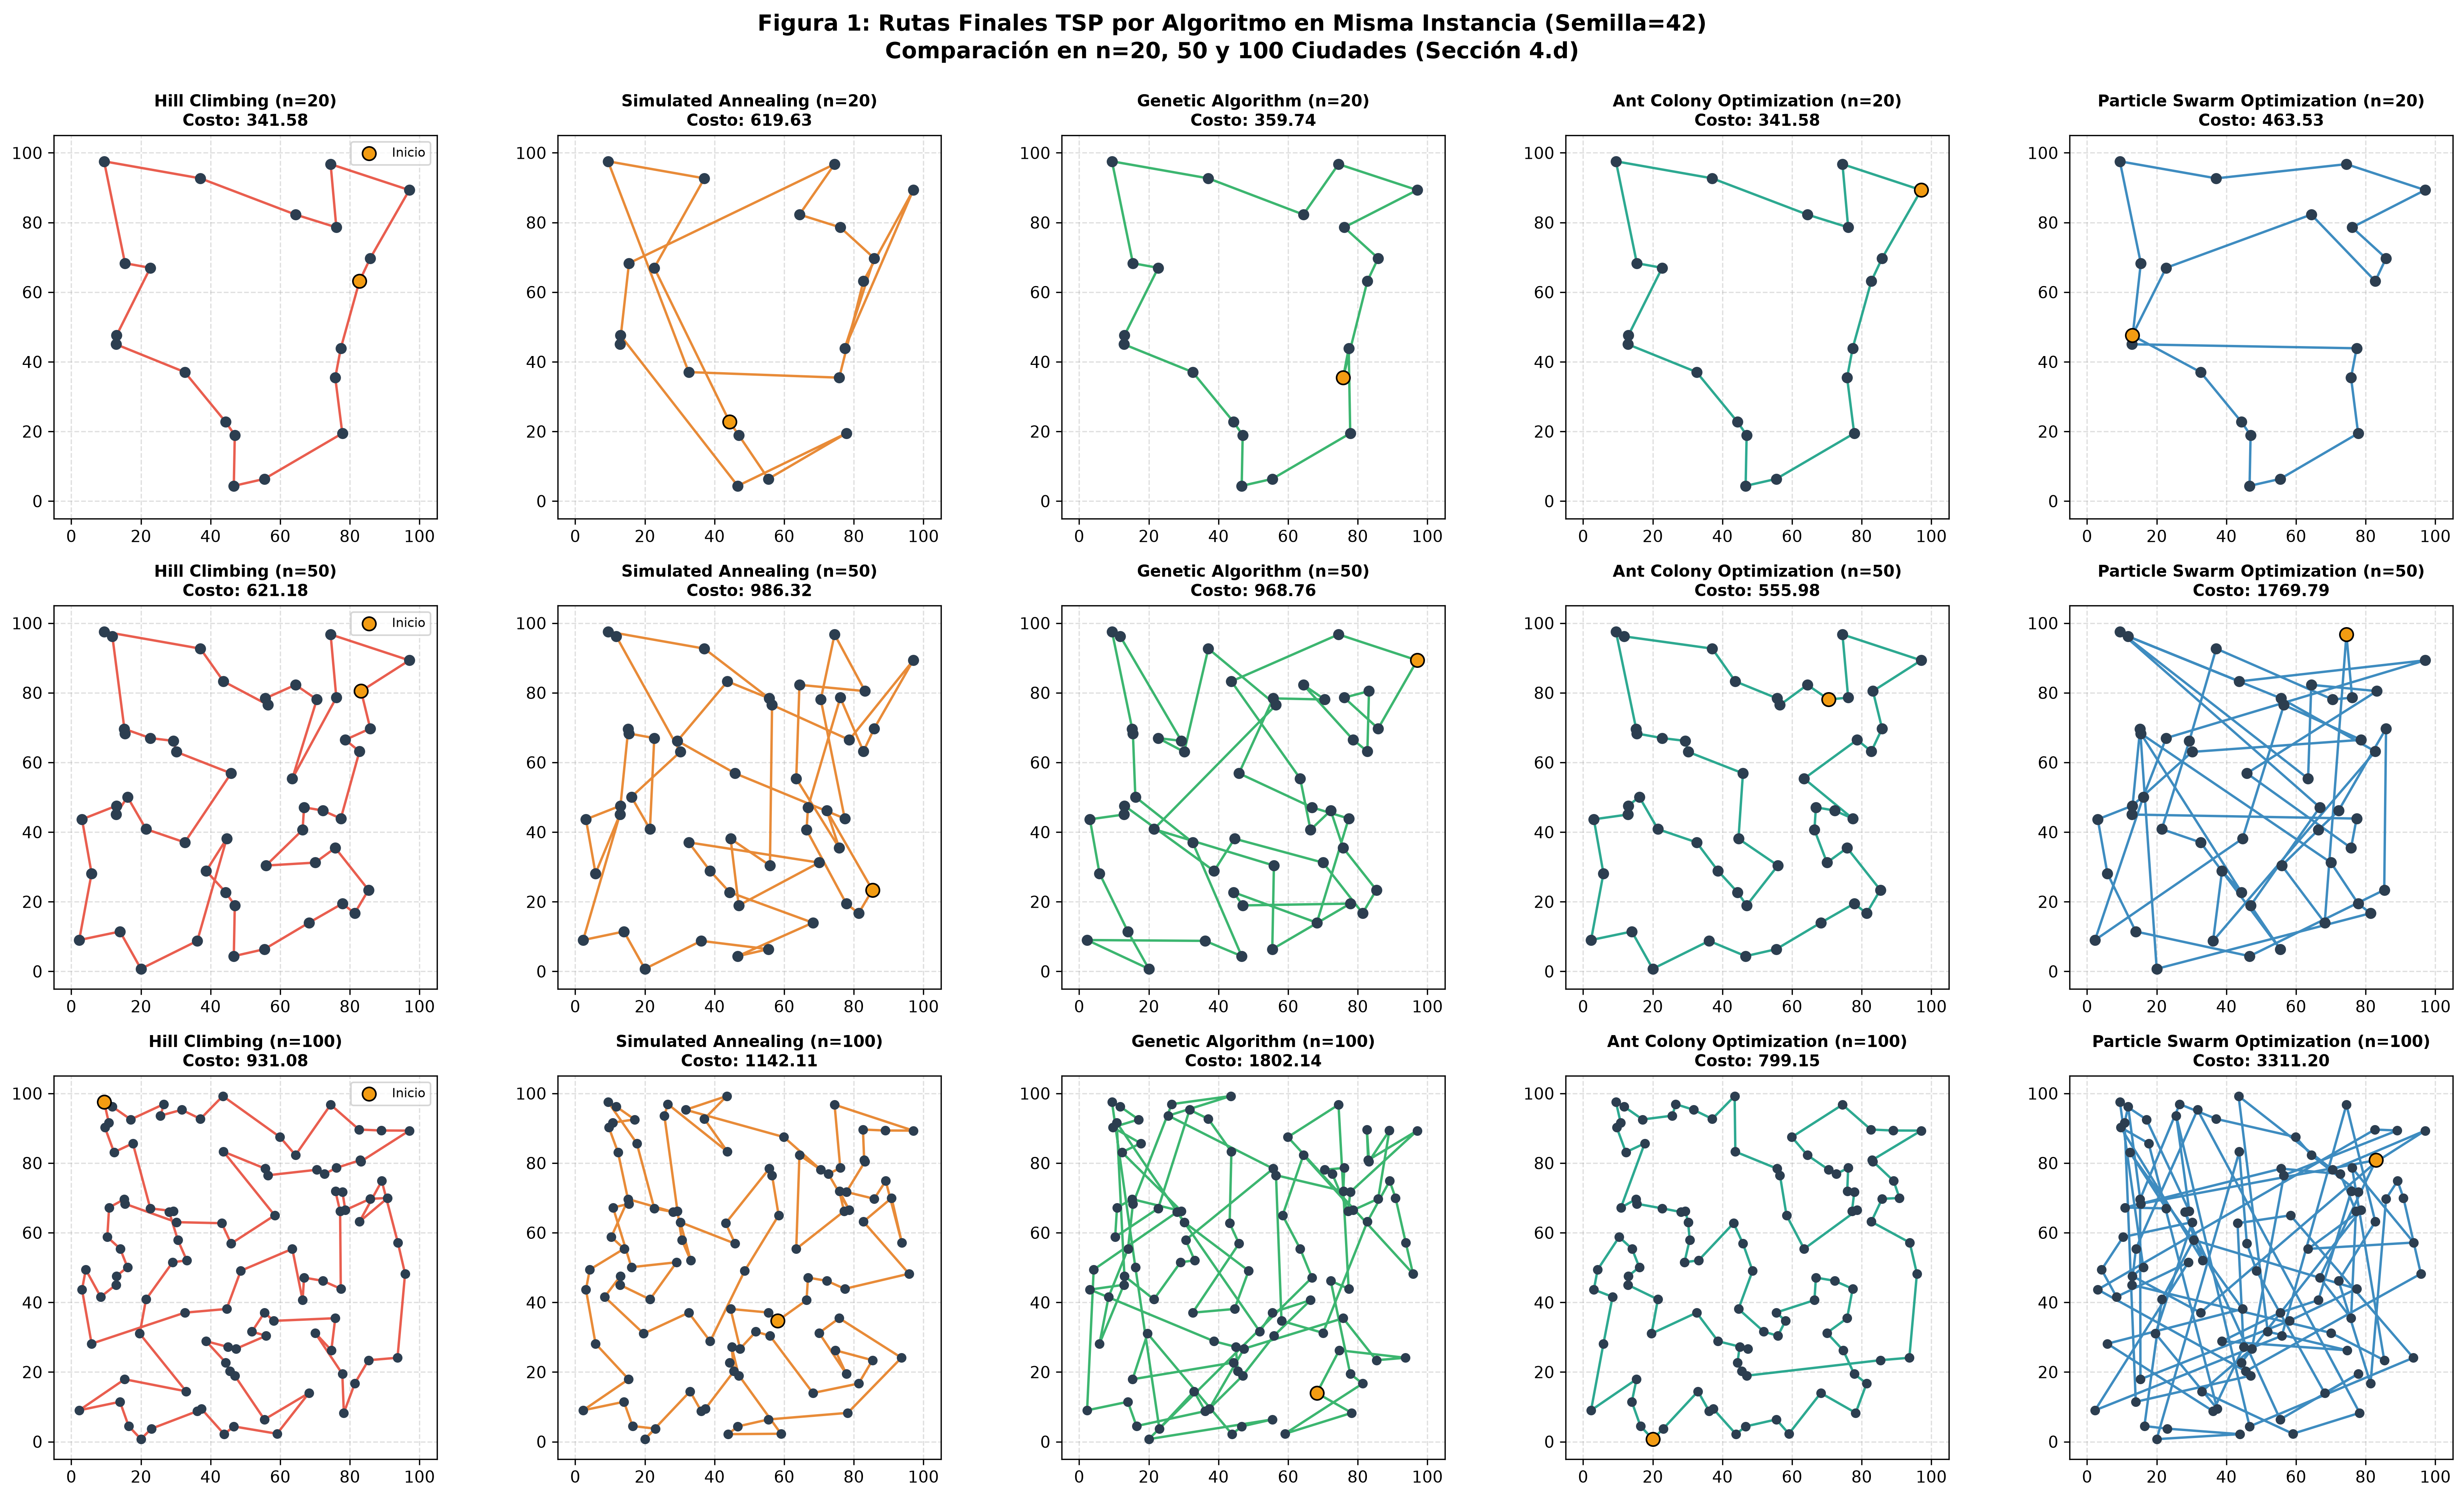
\includegraphics[width=0.98\linewidth]{figuras/01_rutas_comparadas_2d.png}
    \caption{Visualización en el espacio 2D de la mejor ruta encontrada por cada algoritmo ($n=20$). Las aristas cruzadas en SA y PSO delatan subóptimos locales.}
    \label{fig:rutas}
\end{figure}

El análisis geométrico revela que tanto ACO como Hill Climbing lograron rutas convexas sin intersecciones de aristas (costo $341.58$). Por el contrario, Simulated Annealing y PSO presentan múltiples lazos cruzados (aristas que se intersectan), demostrando que fallaron en aplicar movimientos 2-opt correctivos antes de agotar su temperatura o inercia.

\subsection{Ranking Multidimensional Consolidado (Literal 4.e)}
Para jerarquizar el desempeño global se construyó el gráfico de barras multidimensional de la Figura~\ref{fig:ranking}, el cual integra la calidad de solución (menor costo final), la estabilidad (menor desviación típica) y el costo computacional (tiempo de CPU).

\begin{figure}[htbp]
    \centering
    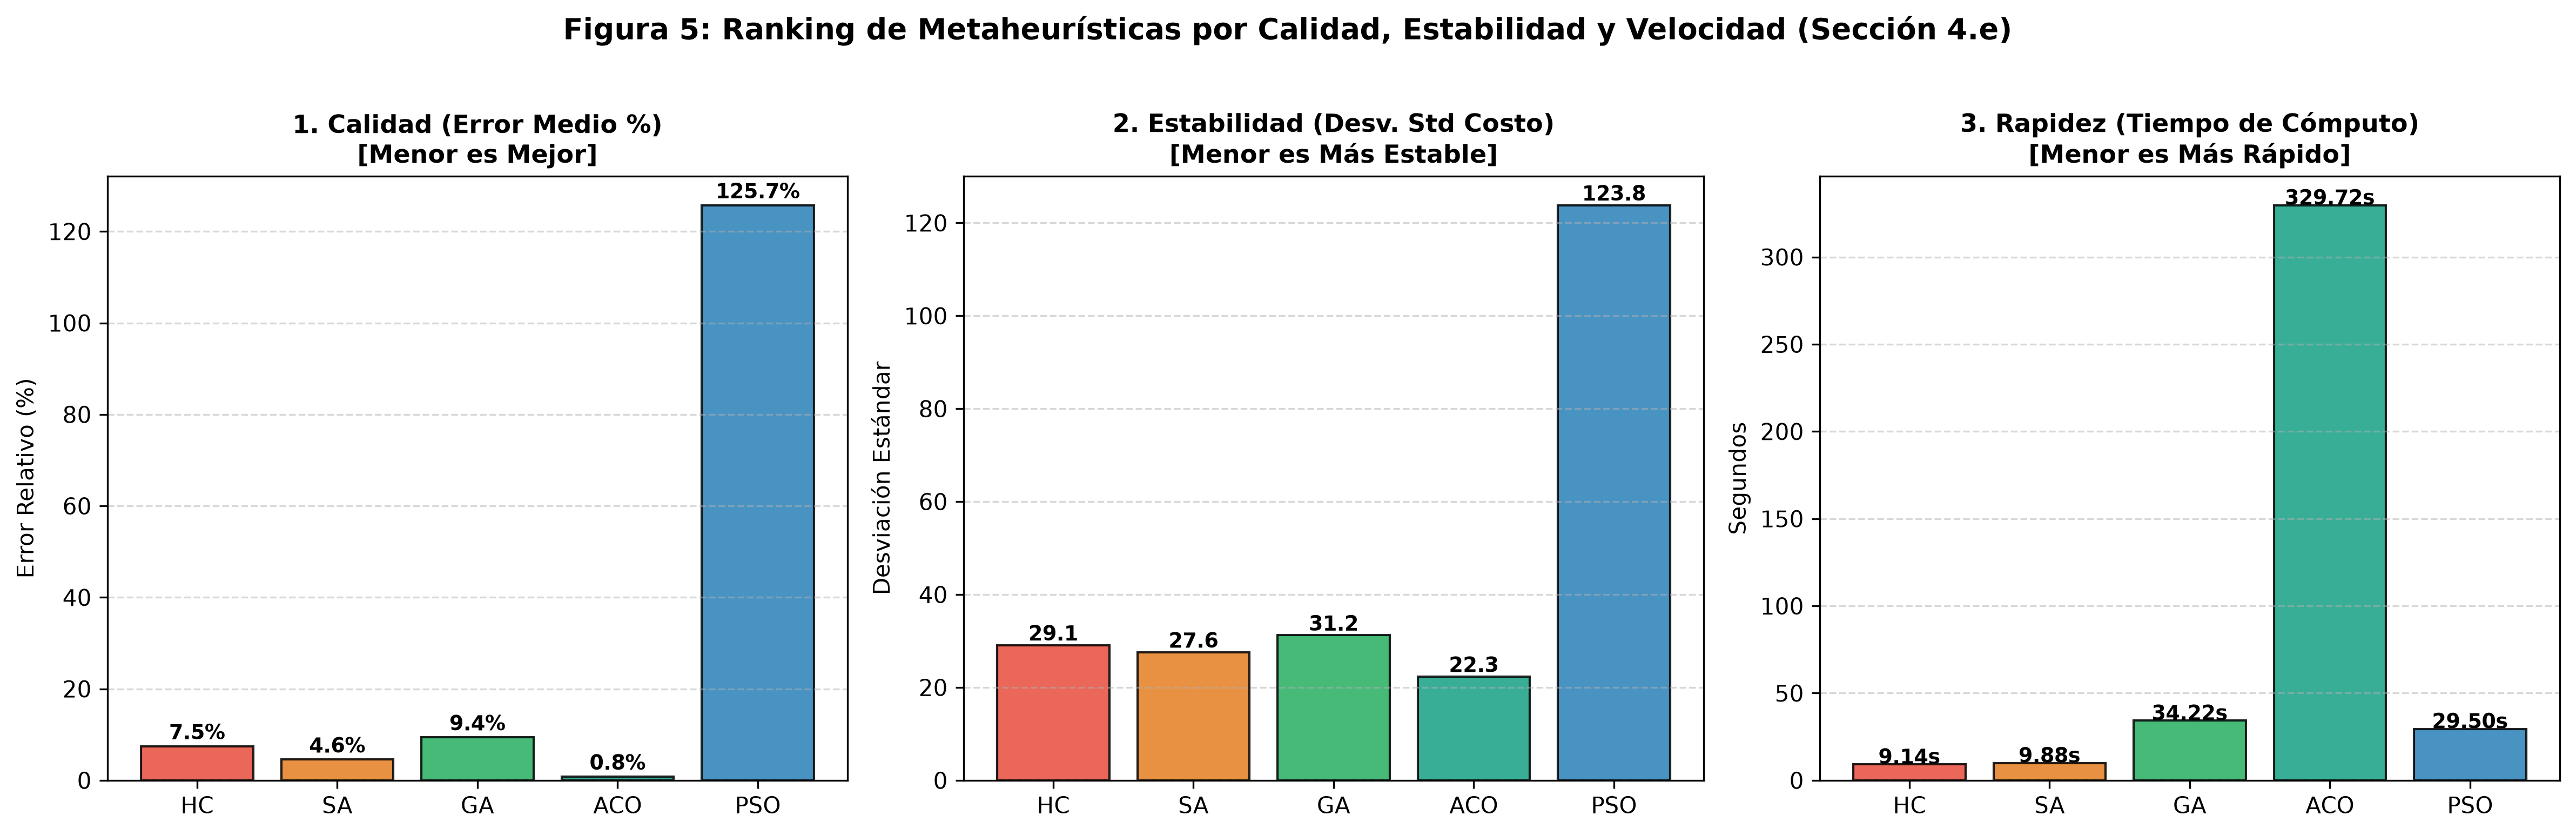
\includegraphics[width=0.92\linewidth]{figuras/05_ranking_calidad_estabilidad_tiempo.png}
    \caption{Ranking multidimensional de los algoritmos: normalización de calidad de ruta, estabilidad y eficiencia en tiempo.}
    \label{fig:ranking}
\end{figure}

El ranking posiciona a \textbf{ACO en el 1.er lugar de Calidad y Estabilidad}, a \textbf{Hill Climbing en el 1.er lugar de Velocidad/Eficiencia}, y sitúa a PSO y SA en las últimas posiciones por deficiencia en la exploración combinatoria discreta.

% =========================================================================
% PUNTO 5: DISCUSIÓN, AMENAZAS A LA VALIDEZ Y CONCLUSIONES
% =========================================================================
\section{Punto 5: Análisis Crítico y Conclusiones}

\subsection{Recomendación de Algoritmos por Escenario de Aplicación}
Con base en la evidencia experimental, se emiten las siguientes directrices de ingeniería:
\begin{itemize}
    \item \textbf{Escenario de Respuesta Rápida en Tiempo Real:} Si se requiere una solución viable en menos de 1 segundo (e.g., reencauzamiento dinámico de entregas o robótica móvil), se recomienda \textbf{Hill Climbing con reinicios aleatorios}. Ofrece rutas competitivas a coste casi nulo de CPU.
    \item \textbf{Escenario de Máxima Calidad y Ahorro Logístico:} Si el objetivo es optimizar costos operacionales de transporte donde un 1\% de combustible representa miles de dólares, se debe implementar \textbf{Ant Colony Optimization (ACO)}, asumiendo el costo temporal de $21$\,s.
    \item \textbf{Escenario con Restricciones de Memoria (Sistemas Embebidos/Edge):} Para microcontroladores o dispositivos IoT con memoria RAM estricta ($< 64$\,KB), \textbf{Hill Climbing} o \textbf{Simulated Annealing} son idóneos al requerir únicamente $\approx 10$\,KB de memoria activa.
\end{itemize}

\subsection{Amenazas a la Validez del Estudio}
\begin{itemize}
    \item \textbf{Validez Interna:} Los hiperparámetros (tasa de evaporación en ACO, enfriamiento en SA, mutación en GA) se mantuvieron fijos durante la ejecución. Un ajuste adaptativo dinámico podría mejorar la convergencia de GA y SA.
    \item \textbf{Validez Externa:} Se evaluaron instancias euclidianas sintéticas en 2D. En matrices asimétricas (ATSP) o redes viales con restricciones de giro y tráfico, la jerarquía de operadores 2-opt podría variar.
\end{itemize}

\subsection{Conclusiones y Trabajo Futuro}
La experimentación demostró que la adaptación de operadores al dominio del problema es más determinante que el paradigma bioinspirado en sí: ACO supera a GA y PSO porque las feromonas depositan conocimiento directamente sobre la matriz de adyacencia del grafo. Como trabajo futuro, se propone una hibridación memética (\textit{ACO + 2-opt local search}) para acelerar la convergencia y mitigar la complejidad temporal en instancias $n \ge 100$.

\end{document}
